\documentclass[master]{suribt}
\usepackage{graphicx}
\usepackage{algorithm}
\usepackage{algorithmicx}
\usepackage{algpseudocode}
\usepackage{amsmath}
\usepackage{amssymb}
\usepackage{amsthm}

\theoremstyle{definition}
\newtheorem{thm}{定理}
\newtheorem{defi}[thm]{定義}
\newtheorem{prop}[thm]{命題}
\newtheorem{cor}[thm]{系}
\newtheorem{asm}[thm]{仮定}

\renewcommand{\algorithmicrequire}{\textbf{Input:}}
\renewcommand{\algorithmicensure}{\textbf{Output:}}
\newcommand{\argmax}{\mathop{\rm argmax}\limits}
\newcommand{\argmin}{\mathop{\rm argmin}\limits}
\newcommand{\tabincell}[2]{\begin{tabular}{@{}#1@{}}#2\end{tabular}}
%\documentclass[oneside]{suribt}% 本文が * ページ以下のときに (掲示に注意)
\title{特許検索における質問意図の曖昧化}
%\titlewidth{}% タイトル幅 (指定するときは単位つきで)
\author{胡瀚林}
\eauthor{HANLIN HU}% Copyright 表示で使われる
\studentid{48-156229}
\supervisor{中川裕志 教授}% 1 つ引数をとる (役職まで含めて書く)
%\supervisor{指導教員名 役職 \and 指導教員名 役職}% 複数教員の場合,\and でつなげる
\handin{2017}{01}% 提出月. 2 つ (年, 月) 引数をとる
%\keywords{キーワード1, キーワード2} % 概要の下に表示される

\begin{document}
\maketitle%%%%%%%%%%%%%%%%%%% タイトル %%%%

\frontmatter% ここから前文
\begin{abstract}%%%%%%%%%%%%% 概要 %%%%%%%%
 企業が特許を取る前に,類似な特許が既に存在するかを確かめるために特許データベースを検索する必要がある.
 しかし,検索の質問から企業秘密が漏洩する可能性がある.
 ウェブテキスト検索の質問からユーザーの検索意図を守る手法が多数存在している.
 その中真の質問と同時にダミー質問を提出する質問曖昧化手法が一番効率的、現実的である.
 本論文では特許検索における既存な質問曖昧化手法\cite{providing2009,embellishing2010,masking2014}を実装し,
 類似度攻撃\cite{simattack2016}で既存手法の安全性を評価した.

 また、類似度攻撃\cite{simattack2016}を含め、多くの既存な質問曖昧化に対する攻撃手法は攻撃者が質問者の事前情報を持つと仮定する.
 本論文では事前情報なしの攻撃手法を提案し,その攻撃手法に対応できる既存な質問曖昧化の改良と新たな質問曖昧化手法を提案する.
\end{abstract}

 \tableofcontents%%%%%%%%%%%%% 目次 %%%%%%%%

 \mainmatter% ここから本文 %%% 本文 %%%%%%%%
 \chapter{はじめに}

 テキスト検索をするとき,検索質問をサーバー側に渡さなければならない.
 しかし,検索質問から質問者の情報が漏洩する危険があることがAOL事件\cite{2006}より証明された.
 特許検索の場合は検索質問が研究開発動向など企業秘密を含んでいるため,一般的なウェブ検索の質問者より質問のプライバシー問題を重視している.
 そのような問題を解く様々な手法が存在している.
 \cite{}や\cite{}などのIPアドレスの匿名化メカニズムは登録情報が必要な検索サーバーに対応できない.
 また検索質問のみから質問者を一意に特定されてしまう可能性がある\cite{2006}.
 プライベート情報検索(Private Information Retrieval )\cite{}は計算量的安全性を持つが,サーバー側で大量の計算が必要であるため実用するのは難しい.
 曖昧化検索(Obfuscation Search)\cite{}は真の質問を分析し適切な$K−1$個のダミー質問を生成し真の質問と同時に検索する.
 安全性が弱いが,効率よく質問者の検索意図を守ることができる.
 %またサーバー側の調整の必要がないため検索結果に影響がない.
 

 本論文の構成は次の通りである.
 第二章では特許文章と特許検索の特徴を述べる.
 第三章では既存な質問曖昧化メカニズム\cite{providing2009,embellishing2010,masking2014}を述べる.
 第四章では曖昧化メカニズムがよく用いる意味分析手法を述べる.
 第五章では既存な攻撃手法\cite{simattack2016}を述べ,\cite{simattack2016}の改良と新たな攻撃手法を提案する.
 第六,七章では新たな質問曖昧化手法を提案する.
 最後に, 第八章で評価実験を述べ,第九章で全体をまとめる.


 \chapter{特許}
 特許検索質問のプライバシーを保護する手法を説明する前に特許検索と特許そのものを簡単に紹介する必要がある.
 特許法第1条には,「この法律は、発明の保護及び利用を図ることにより、発明を奨励し、もつて産業の発達に寄与することを目的とする」とある.
 特許制度は,発明者には一定期間,一定の条件のもとに特許権という独占的な権利を与えて発明の保護を図る一方,
 その発明を公開して利用を図ることにより新しい技術を人類共通の財産としていくことを定めて,
 これにより技術の進歩を促進し,産業の発達に寄与しようというものである.\cite{https://www.jpo.go.jp/seido/s_tokkyo/chizai04.htm}
 特許を取るには以下の条件を満たさなければならない:
 新規性:公知の発明と同様の発明は特許を受けることができない;
 進歩性:先行技術に基づいて容易に発明をすることができる発明は特許を受けることができない.
 単一性:発明の単一性の要件を満たさない二以上の発明は一つの願書で出願することができない.

 特許を受けようとする発明を特定するために特許請求の範囲を記載する必要がある.
 \begin{figure}
  \hspace*{-2cm}
  \begin{tabular}{cc}
  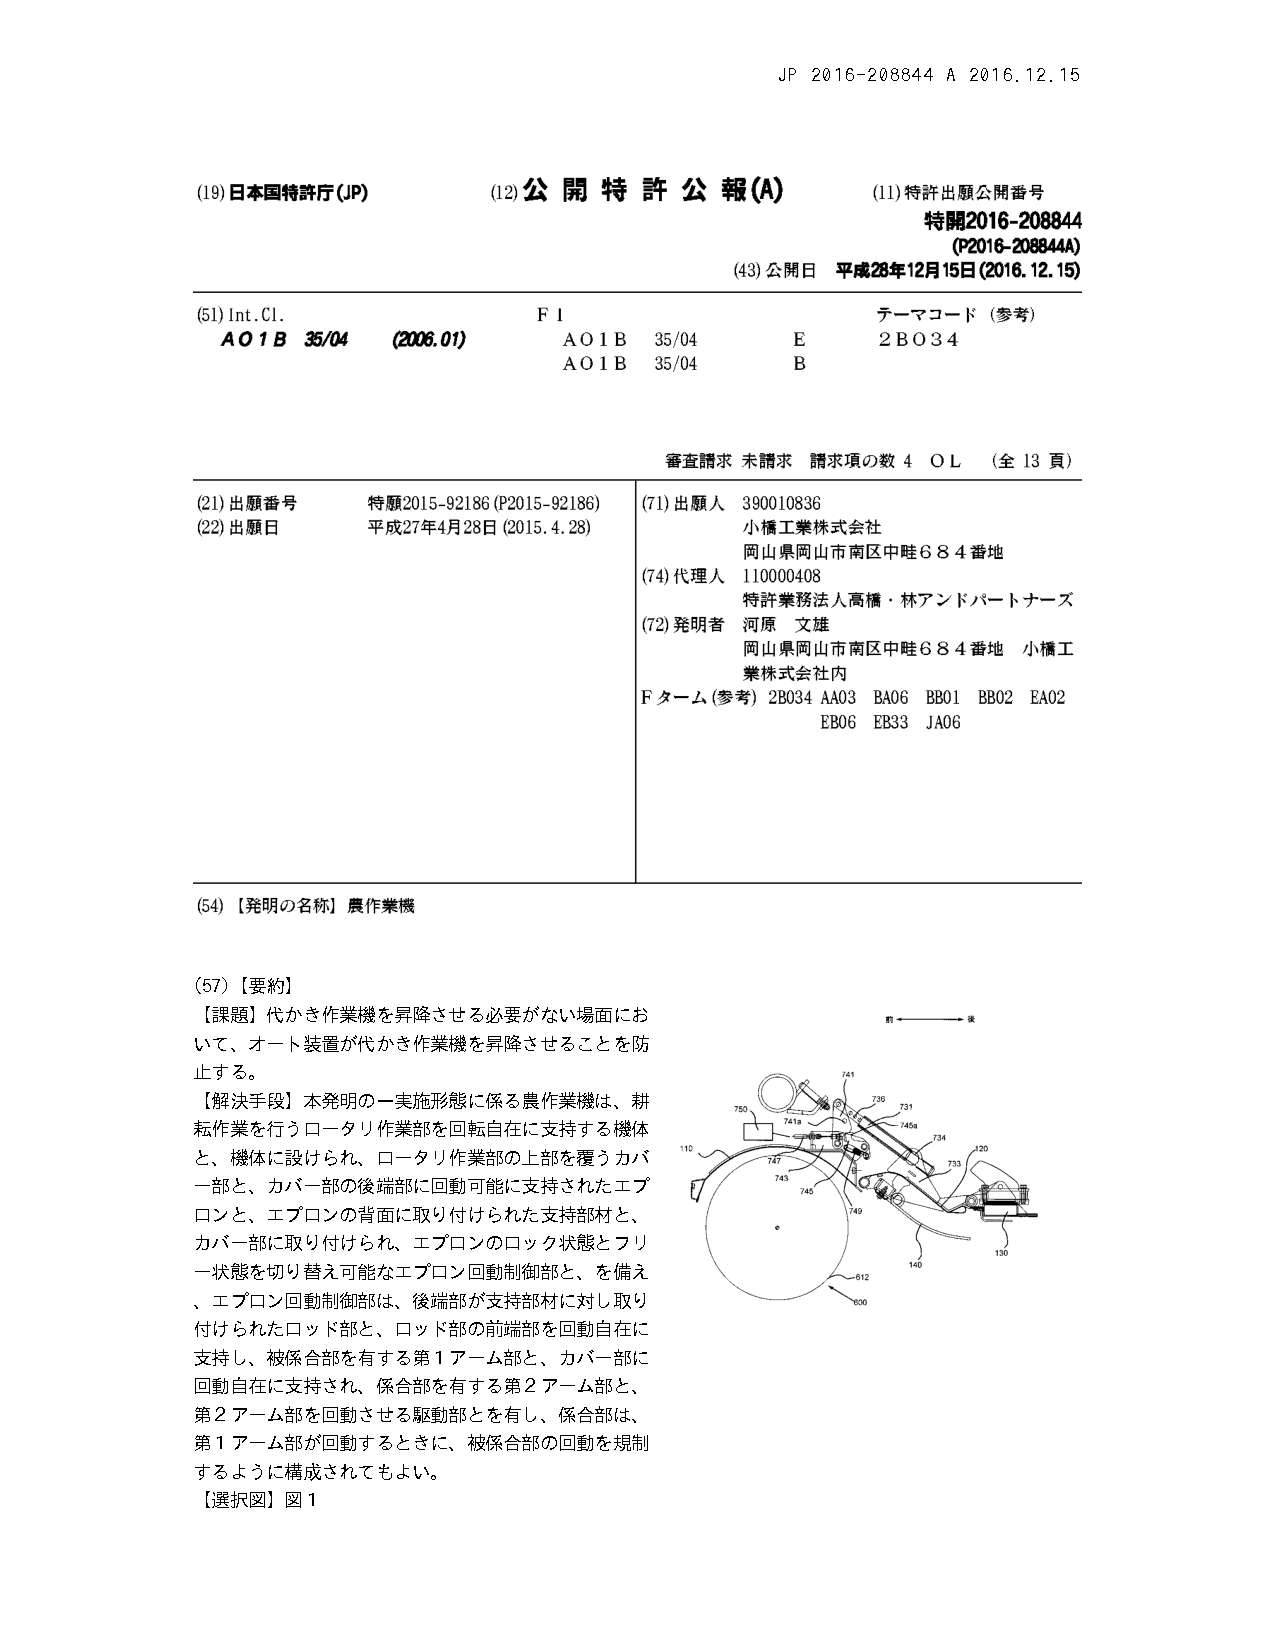
\includegraphics[width=0.55\textwidth,natwidth=500,natheight=1100]{ex1-1.pdf}
  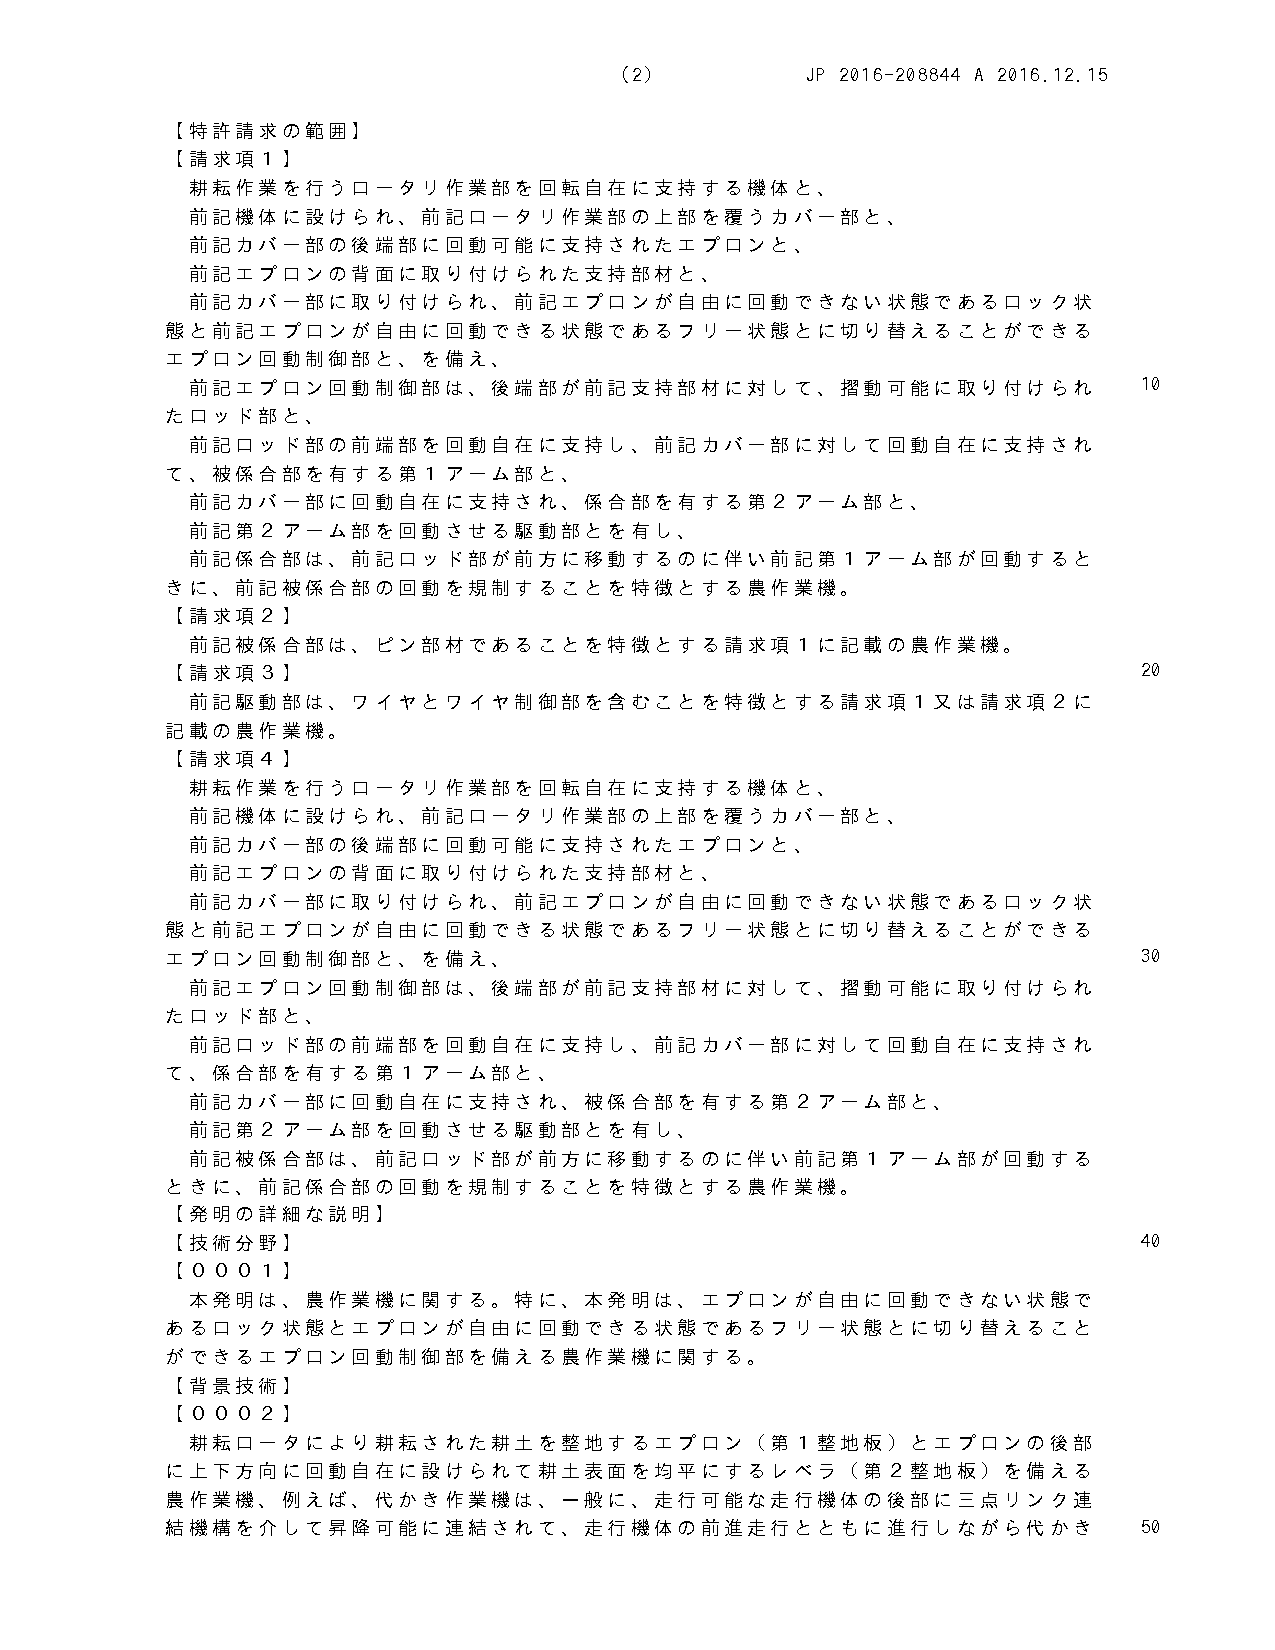
\includegraphics[width=0.55\textwidth,natwidth=500,natheight=1100]{ex1-2.pdf}
  \end{tabular}
  \caption{特許文章例}
  \label{fig:exp}
 \end{figure}

 図\ref{fig:exp}で表した例のように,特許の請求項は特定の書き方がある.
 誤解を招かないように技術用語は、学術用語を用いる.
 また,一般的な文章は単語をなるべく重複しないようにする一方,特許文章は単語を全体を通じて統一して使用する.
 \section{特許分類}
 特許の一つ特徴は全ての特許が人の手によって分類されている.
 特許分類を用いることより検索する特許文章が減り,似たようなキーワードを含むが分類が違う特許文章を排除することができる.
 今最も使われている特許分類が世界知的所有権機関(WIPO)による管理されている国際特許分類(IPC)である.
 国際特許分類は階層構造であり,一番上の階層はAからHまでの8個のセクションである.
 セクション以下は\ref{tab:IPC}に表したように四つの階層に分類されている.
 
 \begin{table}[!hbp]
 \center
 \begin{tabular}{cc}
    セクション:A & 健康および娯楽 \\
    サブセクション : 61 & 医学または獣医学:衛生学 \\
    クラス: C & 歯科:口腔または歯科衛生 \\
    メイングループ:5 & 歯の充填または被覆 \\
    サブグループ:08 & 歯冠:その製造;口中での歯冠固定 \\
 \end{tabular}
 \caption{国際特許分類例:A61C 5/08}
 \end{table}

 \section{特許検索}
 \begin{table}[!hbp]
 \center
 \begin{tabular}{|c|c|c|}
 \noalign{\hrule height 1pt}
 検索タイプー & 検索対象(specification) & 検索目的 \\
 \hline
 \tabincell{c}{技術水準調査\\(State of the Art Search)} & イデア & 自分の発明に関連する背景知識を得る \\
 \tabincell{c}{新規性調査\\(Novelty Search)} & 特許文章 & 特許登録の可能性を判断する \\
 \tabincell{c}{侵害調査\\(Infringement Search)} &  \tabincell{c}{商品と\\商品に関連する技術} & 権利侵害とならないかを判断する \\
 \noalign{\hrule height 1pt}
 \end{tabular}
 \caption{特許検索タイプー}
 \end{table}


 \begin{table}[!hbp]
 \center
 \begin{tabular}{|c|c|}
 \hline
 符号 & 意味 \\
 \hline
 $N$ & 辞書中の単語の数 \\
 $W = \{1,2,3, \dots ,N\} $ & 単語集合 \\
 $M$ & コーパス中の文書の数 \\
 $D = \{1,2,3, \dots ,M\}$ & 文章集合 \\
 $K$ & トピック数 \\
 $T = \{1,2,3, \dots ,K\}$ & トピック集合 \\
 $\ell_i = \{t_1,t_2,\dots,K\} $ & 単語$i$のトピックベクトル \\
 $\ell$ & 質問のトピックベクトル \\
 \hline
 \end{tabular}
 \caption{表記法}
 \end{table}

 \chapter{曖昧化検索}
 曖昧化検索は質問者が検索したい真の質問と質問者側で生成したダミー質問を一緒に検索サーバーに提出し,真の質問がどれかを曖昧化するものである.
 本論文では以下のモデル\cite{}を用いて既存な曖昧化検索メカニズムを分析する.
 質問者Aliceがとある検索サーパ-に質問を出して手に入れたい情報を検索し,
 検索サーバーが semi-honest な攻撃者であることを仮定する.
 
 質問が単語の集合であり,質問の定義域を単語集合の冪集合にする.
 
 \begin{defi}{ユニバーサル質問集合$Q$.}
  $W$を全ての単語の集合とする.
  ユニバーサル質問集合$Q$とは$W$の冪集合である,つまり
  \begin{equation}
  Q = P(W) = \{A|A \subset W\}
  \end{equation}
 \end{defi}
 Aliceのプロフィールを多項分布と仮定し,Aliceが持つ真のプロフィールを$X$とする.
 
 \begin{defi}{質問者のプロフィール$X$.}
  $T$を全てのトピックの集合とする.
  質問者のプロフィール$X$とは
  \begin{equation}
   X = \{x_i| i \in T\}
  \end{equation}
  $x_i$は質問者がトピック$i$に対して持つ興味の強さを表す.
 \end{defi}
 曖昧化検索メカニズムはAliceのコンピュータで実行する.
 曖昧化検索メカニズムが意味分析ツール$S$を用いて真の質問$q_R$を分析しダミー質問$q_D$を生成し,検索サーバーに提出する.
 質問$q$とトピック$t$の関係を表す関数と質問間の距離は以下のように定義する,
 
 \begin{defi}{質問-トピックスコア関数:$rscore_S$.}
  $T$を全てのトピックの集合とする.
  質問$q$とトピック$t$の関係を表す関数とは
  \begin{equation}
   rscore_S:Q \times T \to \mathbb{R}
  \end{equation}
 \end{defi}
 
 \begin{defi}{質問間距離関数:$dist_S$.}
  質問$q_1$と質問$q_2$間の距離を表す関数とは
  \begin{equation}
   dist_S:Q \times Q \to \mathbb{R}
  \end{equation}
 \end{defi}
 
 検索サーバーがAliceからもらった質問をすべて記録し,その質問たちを分析し得るプロフィールを$Y$にする.
 
 曖昧化検索は3つ違うレベルな目的がある.
 まずは質問そのものの曖昧化である.
 質問者が検索した真の質問$q_R$はどの質問であるかをわからないようにする.
 2つ目は質問意図の曖昧化である.
 質問者が検索したいものは何であるかをわからないようにする.
 最後は質問者のプロフィール$X$の曖昧化である.
 $Y$から質問者が興味を持つトピックは何であるかをわからないようにする.
 
 質問の曖昧化ができたとしても質問意図の曖昧化ができると限れない.
 {林檎}と{リンゴ}の2つ質問から真の質問を確定することができないが,質問者が林檎について検索したいことが確定できる.
 同じように{林檎}と{梨}の2つ質問から質問者が検索したいを確定することができないが,質問者が果物に興味を持つことが確定できる.
 本論文では質問意図の曖昧化をメインにする.
 
 \section{否認可能検索を利用したプライバシー保護\cite{providing2009}}
 
 否認可能検索という概念を提出したのは\cite{}である.
 つまり, サーバーは特定なユーザーが特定の時間に提出した一連の質問$L = {q_1, q_2, \dots , q_K}$のログを持つと仮定する. 
 ログにアクセスしたある人が真の検索質問が$q_i$だと証明したいとき, $L$の中の任意の質問$q_j$が真の質問となる確率が同じ$1/K$だと証明できる.
 以下に否認可能検索を定義する.
 \begin{defi}{$k−$否認可能検索}
 	質問$q$をユーザーが入力した質問とする.ダミー質問生成システム$D$が$k$個の質問を含んでいる質問集合$D(q_u)=\{q_1, \dots , q_k\}$を出力しサー
	バーに提出する.$D(q_u)$が以下の性質を持つなら,$D(q_u)$をPD-質問集合といい,$D$を$k$−否認可能検索という
	\begin{enumerate}
	\item $\exists q_i \in D(q_u),q_i$と$q_u$が意味的に近い
	\item $\forall q_j \in D(q_u),D(q_j) = D(q_u)$
	\item $\forall q_j \in D(q_u),q_j$が違うトピックに含まれる
	\item $\forall q_j \in D(q_u),q_j$が同じような尤もらしさを持つ
	\end{enumerate}
  \end{defi}
 \section{質問者のプライバシーを保護する質問加工法\cite{embellishing2010}}
 \section{質問意図を曖昧化するキーワード検索\cite{masking2014}}
 \begin{algorithm}
 \caption{HDGA(On Masking Topical Intent in Keyword Search)}
 \begin{algorithmic}[1]
  \Require 質問:$q_1$
  \State $Q = \{q_1\}\delta_{q_1} = \argmax_{t \in T} Pr[t|q_1]$
  \ForAll {$t \in T \setminus \{\delta_{q_1}\}$}
  \State $e_t = h(\delta_{q_1}||t||s)$
  \EndFor
  \State $T_D = \{t^1_{q1},t^2_{q1}, \dots , t^2_{q1} | \forall t_1 \ \in T_D , \forall t_2 \ \in T \setminus T_D, e_{t_1} > e_{t_2} \}$
  \ForAll {$t \in T_D $}
  \While { $ \argmax_{t \in T} Pr[t|q'] \neq t$}
  \State randomly select $|q_1|$ keywords for $t$ based on $Pr[w|t]$, to form a dummy query $q'$
  \EndWhile
  \State $Q = Q \cup \{q'\}$
  \EndFor 
  \State Shuffle queries in Q
  \Return $Q$
 \end{algorithmic}
 \end{algorithm}

 \chapter{意味分析}
 \section{tf-idf}
 \section{潜在意味解析}
 \section{潜在的ディリクレ配分法}
 \chapter{プライバシー分析(攻撃手法)}
 \section{メイントピック攻撃}
 \begin{algorithm}
 \caption{メイントピック攻撃}
 \begin{algorithmic}[1]
  \Require 質問:$q=\{t_i\},$単語のトピックベクトル集合$L=\{\ell_i\}$
  \State $R=\phi, \, \ell=0$
  \State $\ell=\sum_{t_i \in Q}\ell_{t_i}$
  \State $maintopic = \argmax_j \ell[j]$
  \ForAll {$bk_k \in q $}
  \State $R=R \cup \{\max_{t_i}l_{t_i}[maintopic]\}$
  \EndFor \\
  \Return $R$
 \end{algorithmic}
 \end{algorithm}

 \section{類似度攻撃\cite{simattack2016}(事前情報あり)}
 \begin{algorithm}
 \caption{類似度計算}
 \begin{algorithmic}[1]
  \Require 質問$q$,ユーザープロフィール$P_u$,スムージングパラメータ:$\alpha$
  \For {$q_i \in P_u$}
  \State $coef[i] \leftarrow 2 \cdot |q \cap q_i| \cdot \frac{1}{|q|+|q_i|}$
  \EndFor
  \State $coef \gets sort(coef)$
  \State $sim \gets coef[0]$
  \For {$i \in [1,|P_u|]$}
  \State $sim \gets \alpha \cdot coef[i] + (1 - \alpha) \cdot sim$
  \EndFor
  \Ensure $sim$
 \end{algorithmic}
 \end{algorithm}
 
 \begin{algorithm}
 \caption{類似度攻撃}
 \begin{algorithmic}[1]
   \Require 質問集合$Q$,ユーザープロフィール$Pu$,スムージングパラメータ:$\alpha$
   \State $q^* = \argmax_{q \in Q}sim_{q,Pu}$
   \Ensure $q^*$
 \end{algorithmic}
 \end{algorithm}

 \section{類似度攻撃2(事前情報なし)}

 \begin{algorithm}
 \caption{類似度攻撃}
 \begin{algorithmic}[1]
  \Require 質問集合列$\hat{Q}=\{ Q_1,Q_2, \dots , Q_n\}$,スムージングパラメータ:$\alpha$
  \For {$j \in |Q_1|$}
   \State $\hat{Pu}[j] = Q_1[j]$
   \State $\hat{Put}[j] = \Phi$
   \State $d[j] = 0$
  \EndFor
  \For {$i \in [2,n]$}
   \For {$j \in |Q_i|$}
   \ State $\hat{Put}[j] = \argmax_{Pu \in \hat{Put}}sim_{Q_i[j],\hat{Put}[j]}$
   \EndFor
   \State $q^*_i = \argmin_{Q_i[j] \in Q_i}sim_{Q_i[j],\hat{Put}[j]}$
   \For {$j \in |Q_i|$}
    \State $\hat{Pu}[j] = \hat{Put}[j] \cap Q_i[j]$
   \EndFor
  \EndFor
  \Ensure $q^*$
 \end{algorithmic}
 \end{algorithm}
 
 \chapter{質問曖昧化(提案手法)}
 事前に単語をグループにする\cite{embellishing2010},質問をグループにする\cite{providing2009}と同じようにトピックをグループにすることよりトピック出現頻度で質問者が興味あるトピックを特定することが防ぐと考えられる.
 
 \cite{masking2014}ではハッシュ関数でトピックをグループにしているが,各トピック間の関係を配慮していない.
 また,\cite{masking2014}では各ダミートピックから単語をランダムに選ぶため,
 真の質問に含まれている単語は違っても属するトピックは同じなら
 ダミー質問が同じような性質を持つ。
 一方,同じ真の質問に対して同じダミー質問を生成することができない.
 真の質問に含まれている単語という情報を用いてないことが\cite{masking2014}に提案した手法がSimattackに弱い原因だと考えられる.
 simattackから真の質問を守るために真の質問が同じ単語を含むとき,
 ダミー質問も同様に同じ単語を含んでほしい.
 それを実現するため提案手法では単語ベクトルを用いた.
 
 \section{単語ベクトル}
 
 \begin{defi}{単語ベクトル}
  $T$を全てのトピックの集合とし$W$を全て単語の集合とする.
  トピック$t$の単語ベクトル$l_t$とは
  \begin{equation}
  \begin{aligned}
   & l_t  = \{w_1,w_2, \dots , w_{|W|}\}, \\
   & \forall w \in l_t, w \in W \\
   & \forall  1 \leq i \neq j \leq, w_i \neq w_j \\
   & \forall 1 \leq i < j \leq |W|,rscore(w_i,t) \geq rscore(w_j,t) 
  \end{aligned}
  \end{equation}
 \end{defi}
 質問のメイントピックを計算し,
 質問に含まれている単語をその単語が質問のメイントピックの単語ベクトルにいる順番にすれば,
 質問を数字ベクトルで表わすことができる.
 同様にトピックが決めれば,
 そのトピックの単語ベクトルを用いて数字ベクトルを質問に翻訳することができる.
 
 単語ベクトル内の単語が単語とそのトピックの関連値の大きい方から小さい方までに並ぶため,
 単語ベクトルに同じ順番を持つ単語
 がその単語ベクトルを持つトピックに対して同じ様な関連性を持つと考えられる.
 また,同じ数字ベクトルで表わせる質問も
 その質問が属するトピックに対して同じ様な関連性を持つと考えられる.
 
 したがって,単語ベクトルを通じて違うトピックに属するが似たような特徴を持つ質問を作るこたができる.
 
 
 \section{質問曖昧化}
 
 \chapter{データベース分割}
 特許分類を用いることにより特許データベースを分割することができる.
 分割したデータベース各々に対して同じような信憑性を持つ質問を提出すると真に検索したいデータベースを隠すことができると考えられる.

 \chapter{評価実験}
 \section{データベース}
 \section{tfidf vs lda vs lsa}
 \section{データベース分割}

 \section{検索結果分析(真の質問が当たられる確率 vs ダミー質問と真の質問の検索結果の類似度)}
 \chapter{おわりに}

 \backmatter% ここから後付
 \chapter{謝辞}%%%%%%%%%%%%%%% 謝辞 %%%%%%%

  %\begin{thebibliography}{}%%%% 参考文献 %%%
  % \bibitem{}
  %\end{thebibliography}
  \bibliographystyle{tieice}%           BibTeX を使う場合
  \bibliography{thesis}% BibTeX を使う場合

  \appendix% ここから付録 %%%%% 付録 %%%%%%%
  \chapter{}
  \end{document}
